\section*{Úkol 1}
\label{sec:task-1}

Pomocí nástrojů explorační analýzy zkoumejte nárůst výkonnostních skóre (FPS) po aplikaci 1.5 patche 
(tj. rozdíl výkonnostních skóre pro verzi „patched“ a verzi „release“) ve hře "Cyberpunk 2077" pro grafické karty 
Nvidia RTX 3070 Ti a AMD Radeon RX 7700 XT. Data vhodně graficky prezentujte (krabicový graf, histogram, q-q graf) 
a doplňte následující tabulku a text.

\vspace{2em}
\noindent
Výsledky popisné statistiky lze vidět v \tabref{tab:characteristics-summary} a na Obr. \ref{fig:boxplot_outliers}, \ref{fig:boxplot_without_outliers}, \ref{fig:qq_graph_histogram_rtx_3070_ti}, \ref{fig:qq_graph_histogram_rx7700xt}.

% Fill your table values here :)
\newcommand{\rangeValues}       {65, 65, 64, 61}
\newcommand{\minValues}         {4.2, 3.2, 4.2, 4}
\newcommand{\QfValues}          {5.30, 4.90, 5.275, 4.900}
\newcommand{\medianValues}      {5.70, 5.30, 5.700, 5.200}
\newcommand{\meanValues}        {5.85, 5.46, 5.713, 5.277}
\newcommand{\QtValues}          {6.20, 5.60, 6.200, 5.600}
\newcommand{\maxValues}         {14.7, 16.0, 7.5, 6.6}
\newcommand{\sdValues}          {1.34, 1.50, 0.736, 0.579}
\newcommand{\cvValues}          {22.8, 27.3, 12.9, 11.0} %??????
\newcommand{\skewnessValues}    {4.5, 5.5, 0.0, 0.3}
\newcommand{\kurtosisValues}    {28.1, 36.7, -0.4, 0.0}
\newcommand{\lowerBoundValues}  {3.95, 3.85, 0, 0}
\newcommand{\upperBoundValues}  {7.55, 6.65, 0, 0}


%\newcommand{\rangeValues}       {65, 65, 64, 61}
%\newcommand{\minValues}         {4.2, 3.2, 4.2, 4}
%\newcommand{\QfValues}          {5.3, 4.9, 5.275, 4.9}
%\newcommand{\medianValues}      {5.7, 5.3, 5.7, 5.2}
%\newcommand{\meanValues}        {5.850769, 5.46, 5.7125, 5.27704918}
%\newcommand{\QtValues}          {6.2, 5.6, 6.2, 5.6}
%\newcommand{\maxValues}         {14.7, 16, 7.5, 6.6}
%\newcommand{\sdValues}          {1.332423, 1.492041, 0.7356025, 0.57861716}
%\newcommand{\cvValues}          {22.773466, 27.326765, 12.8770687, 10.96478613}
%\newcommand{\skewnessValues}    {4.515606, 5.485538, -0.0124799, 0.27550042}
%\newcommand{\kurtosisValues}    {28.136639, 36.697488, -0.3643407, -0.02777256}
%\newcommand{\lowerBoundValues}  {3.9499999, 3.85, 0, 0}
%\newcommand{\upperBoundValues}  {7.55000000000001, 6.65000000000001, 0, 0}



% Additional values
% not rounded  {4.241295, 7.183705, 4.119815, 6.434283}
\newcommand{\sigmaValues}       {4.241, 7.184, 4.120, 6.434}

% Helper command to put everything in table.
\newcommand{\tableValue}[2]{%
    \pgfmathparse{{#1}[#2]}%
    \mbox{\pgfmathresult}%
}

\begin{table}[h!]
    \caption{Nárůst výkonnostních skóre (FPS) po aplikaci 1.5 patche ve hře "Cyberpunk 2077" pro grafické karty Nvidia RTX 3070 Ti a AMD Radeon RX 7700 XT (souhrnné statistiky)}
    \label{tab:characteristics-summary}
    \vspace{0.5em}
    \renewcommand{\arraystretch}{1.3}
    \resizebox{\textwidth}{!}{%
        \begin{tabular}{|p{3.5cm}|P{3cm}|P{3cm}|P{3cm}|P{3cm}|}
            \hline
            & \multicolumn{2}{P{6cm}|}{\textbf{Původní data}} & \multicolumn{2}{P{6cm}|}{\textbf{Data po odstranění odlehlých pozorování}} \\ \hline
            & \centering \textbf{Nvidia RTX 3070 Ti} & \textbf{AMD Radeon RX 7700 XT} & \centering \textbf{Nvidia RTX 3070 Ti} & \textbf{AMD Radeon RX 7700 XT} \\ \hline
            rozsah souboru        & \tableValue{\rangeValues}{0}    & \tableValue{\rangeValues}{1}    & \tableValue{\rangeValues}{2}    & \tableValue{\rangeValues}{3}    \\ \hline
            minimum               & \tableValue{\minValues}{0}      & \tableValue{\minValues}{1}      & \tableValue{\minValues}{2}      & \tableValue{\minValues}{3}      \\ \hline
            dolní kvartil         & \tableValue{\QfValues}{0}       & \tableValue{\QfValues}{1}       & \tableValue{\QfValues}{2}       & \tableValue{\QfValues}{3}       \\ \hline
            medián                & \tableValue{\medianValues}{0}   & \tableValue{\medianValues}{1}   & \tableValue{\medianValues}{2}   & \tableValue{\medianValues}{3}   \\ \hline
            průměr                & \tableValue{\meanValues}{0}     & \tableValue{\meanValues}{1}     & \tableValue{\meanValues}{2}     & \tableValue{\meanValues}{3}     \\ \hline
            horní kvartil         & \tableValue{\QtValues}{0}       & \tableValue{\QtValues}{1}       & \tableValue{\QtValues}{2}       & \tableValue{\QtValues}{3}       \\ \hline
            maximum               & \tableValue{\maxValues}{0}      & \tableValue{\maxValues}{1}      & \tableValue{\maxValues}{2}      & \tableValue{\maxValues}{3}      \\ \hline
            směrodat. odchylka    & \tableValue{\sdValues}{0}       & \tableValue{\sdValues}{1}       & \tableValue{\sdValues}{2}       & \tableValue{\sdValues}{3}       \\ \hline
            variační koefi. (\%)  & \tableValue{\cvValues}{0}       & \tableValue{\cvValues}{1}       & \tableValue{\cvValues}{2}       & \tableValue{\cvValues}{3}       \\ \hline
            šikmost               & \tableValue{\skewnessValues}{0} & \tableValue{\skewnessValues}{1} & \tableValue{\skewnessValues}{2} & \tableValue{\skewnessValues}{3} \\ \hline
            špičatost             & \tableValue{\kurtosisValues}{0} & \tableValue{\kurtosisValues}{1} & \tableValue{\kurtosisValues}{2} & \tableValue{\kurtosisValues}{3} \\ \hline
            \multicolumn{5}{|p{16cm}|}{\textbf{Identifikace odlehlých pozorování (vnitřní hradby)}} \\ \hline
            dolní mez   & \tableValue{\lowerBoundValues}{0} & \tableValue{\lowerBoundValues}{1} & \multicolumn{2}{P{6cm}|}{------------} \\ \hline
            horní mez   & \tableValue{\upperBoundValues}{0} & \tableValue{\upperBoundValues}{1} & \multicolumn{2}{P{6cm}|}{------------} \\ \hline
        \end{tabular}%
    }
\end{table}

\newpage
\noindent
\textbf{Grafická prezentace (krabicový graf, histogram, q-q graf)}

\begin{figure}[h!]
    \centering
    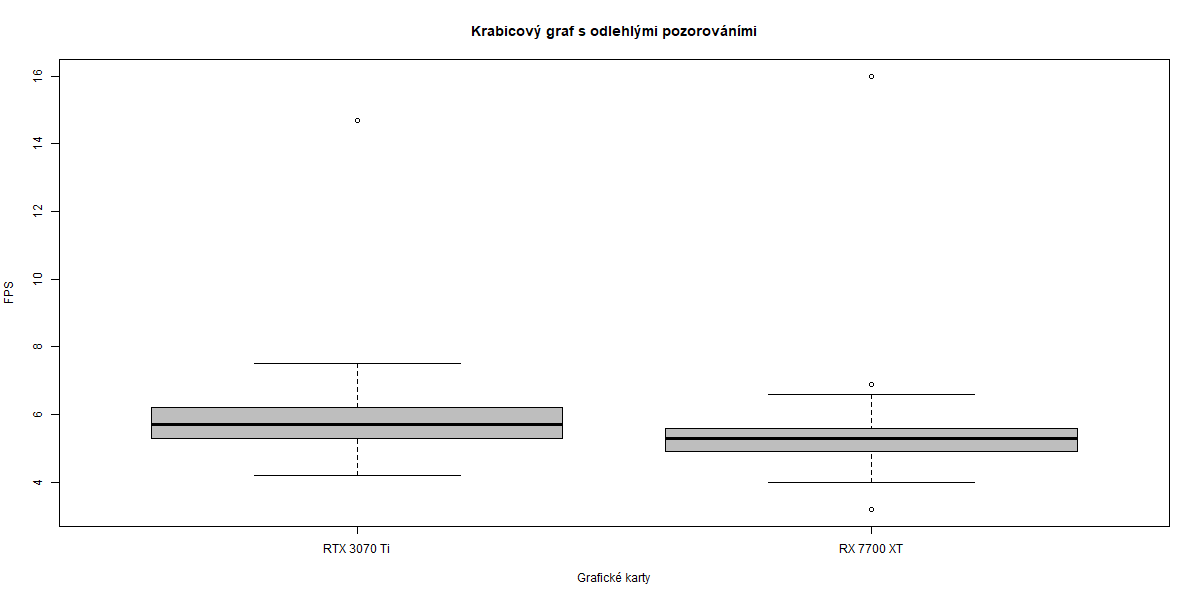
\includegraphics[width=1.00\textwidth]{assets/boxplot_outliers.png}
    \caption{ Nárůst FPS po aplikaci patche 1.5 ve hře Cyberpunk 2077 (krabicový graf, původní data) }
    \label{fig:boxplot_outliers}
\end{figure}



\begin{figure}[h!]
    \centering
    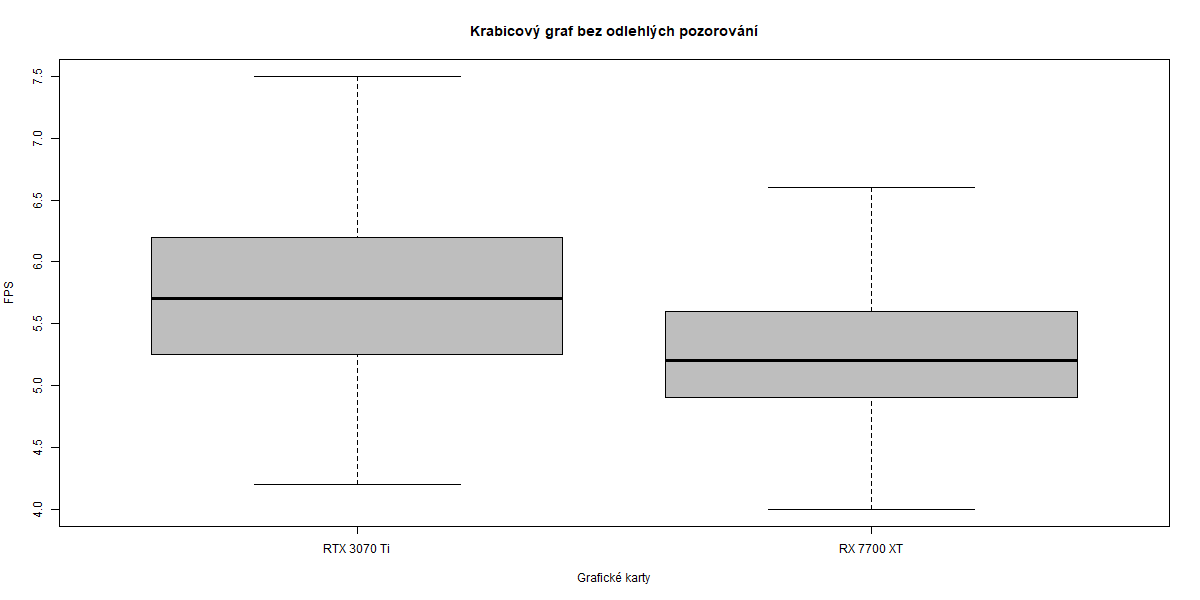
\includegraphics[width=1.00\textwidth]{assets/boxplot_without_outliers.png}
    \caption{ Nárůst FPS po aplikaci patche 1.5 ve hře Cyberpunk 2077 (krabicový graf, data bez odlehlých pozorování) }
    \label{fig:boxplot_without_outliers}
\end{figure}



\begin{figure}[h!]
    \centering
    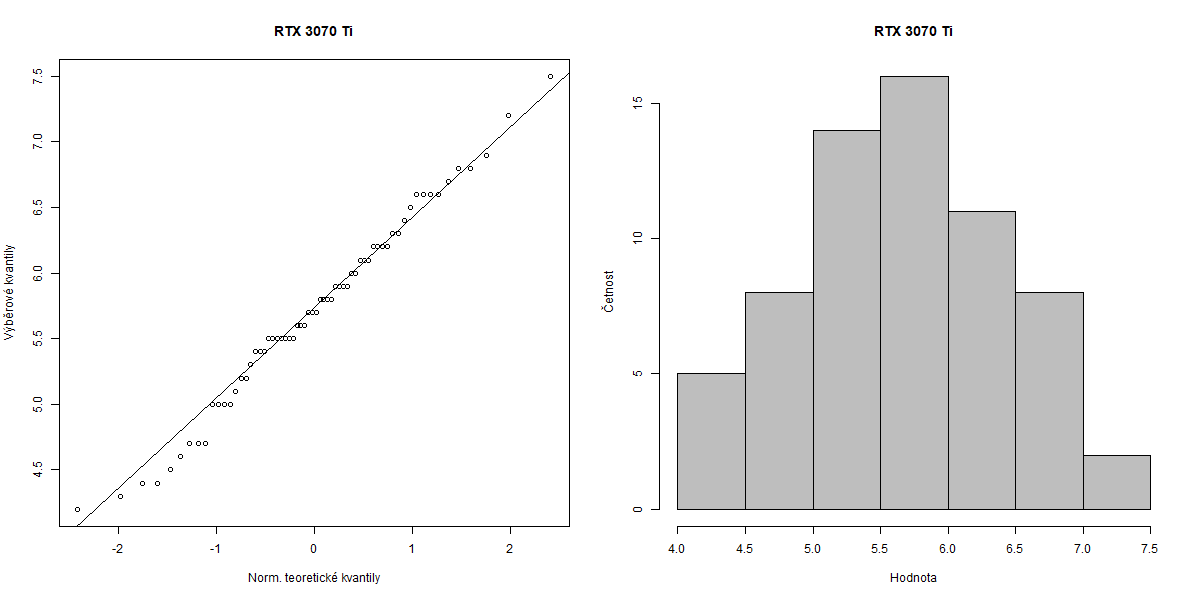
\includegraphics[width=1.10\textwidth]{assets/combined_qq_histogram_rtx3070ti.png}
    \caption{Nárůst FPS po patchi 1.5 ve hře Cyberpunk 2077 pro grafickou kartu RTX 3070 Ti (data po
    odstranění odlehlých pozorování)}
    \label{fig:qq_graph_histogram_rtx_3070_ti}
\end{figure}


\begin{figure}[h!]
    \centering
    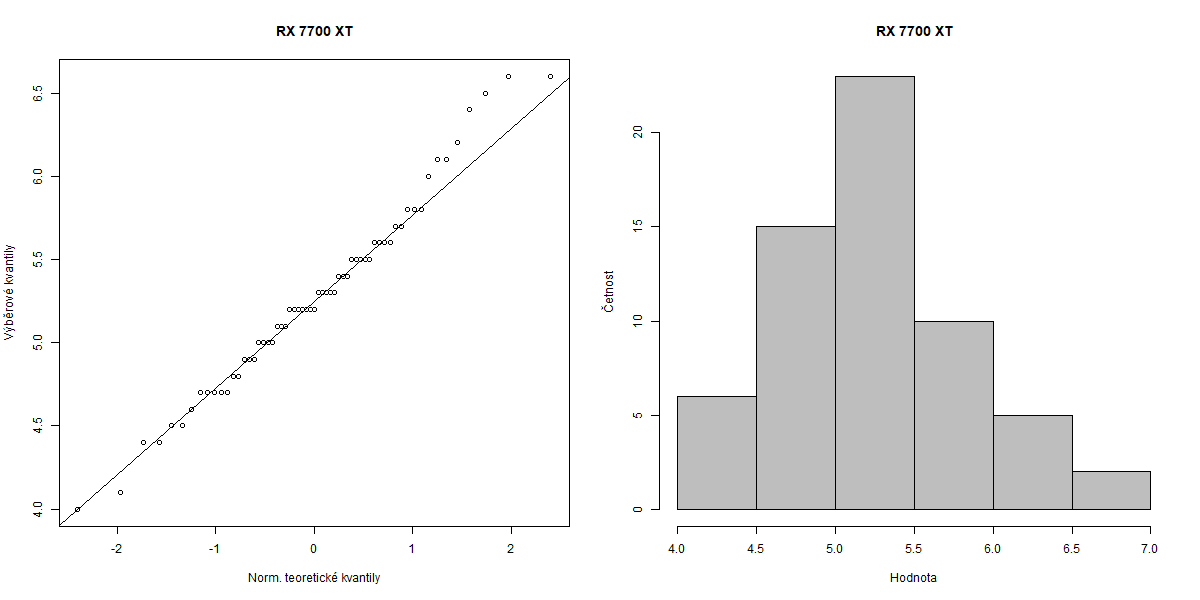
\includegraphics[width=1.10\textwidth]{assets/combined_qq_histogram_rx7700xt.png}
    \caption{Nárůst FPS po patchi 1.5 ve hře Cyberpunk 2077 pro grafickou kartu RX 7700 XT (data po
    odstranění odlehlých pozorování)}
    \label{fig:qq_graph_histogram_rx7700xt}
\end{figure}





\newpage
\subsubsection*{Analýza nárůstu výkonnostních skóre (FPS) po aplikaci 1.5 patche ve hře "Cyberpunk 2077" pro grafickou kartu Nvidia RTX 3070 Ti}

% TODO: Solve underline questions.
Během testu byl zjišťován nárůst FPS pro grafickou kartu Nvidia RTX 3070 Ti ve hře "Cyberpunk 2077" mezi původním release a verzí s 1.5 patchem 
pro \tableValue{\rangeValues}{0} testovacích systémů. Zjištěný nárůst FPS se pohyboval v rozmezí \tableValue{\minValues}{0} FPS
až \tableValue{\maxValues}{0} FPS. Nárůst FPS v testu č. 37 byl na základě metody vnitřních hradeb identifikován jako odlehlé pozorování
a nebude zahrnut do dalšího zpracování. \footnote{V případě potřeby (existence vícero odlehlých pozorování) větu vhodným způsobem upravte.}
Možné příčiny vzniku odlehlých pozorování jsou: Náhlé výkyvy výkonu měřené sestavy nebo chyba měřícího softwaru. Dále uvedené výsledky 
tedy pocházejí z analýzy nárůstů FPS zjištěných u \tableValue{\rangeValues}{2} testovacích systémů. Průměrný nárůst FPS byl \tableValue{\meanValues}{2} FPS, 
směrodatná odchylka pak \tableValue{\sdValues}{2} FPS. U poloviny testovacích cyklů nárůst FPS nepřekročil \tableValue{\medianValues}{2} FPS\@.
V polovině případů se nárůst FPS pohyboval v rozmezí \tableValue{\QfValues}{2} FPS až \tableValue{\QtValues}{2} FPS. Vzhledem k hodnotě
variačního koeficientu (\mbox{\tableValue{\cvValues}{2}}\%) lze analyzovaný soubor považovat za homogenní.

\vspace{1em}
\noindent
Výsledky pro grafickou kartu AMD Radeon RX 7700 XT lze komentovat obdobně.

\subsubsection*{Ověření normality nárůstu výkonnostních skóre (FPS) po aplikaci 1.5 patche ve hře "Cyberpunk 2077" pro grafickou kartu Nvidia RTX 3070 Ti}

% TODO: Solve underline questions.
Na základě grafického zobrazení (viz. Obr. \ref{fig:boxplot_without_outliers} a \ref{fig:qq_graph_histogram_rtx_3070_ti}) a výběrové šikmosti a špičatosti (viz \tabref{tab:characteristics-summary}, výběrová šikmost a špičatost leží 
v intervalu (-2, 2)) lze  předpokládat, že pozorovaný nárůst FPS má normální rozdělení. Dle pravidla 3$\sigma$
lze tedy očekávat, že přibližně u 95 \% naměřených nárůstů ve výkonu bude \tableValue{\sigmaValues}{0} FPS až \tableValue{\sigmaValues}{1} FPS\@.

\subsubsection*{Ověření normality nárůstu výkonnostních skóre (FPS) po aplikaci 1.5 patche ve hře "Cyberpunk 2077" pro grafickou kartu AMD Radeon RX 7700 XT}

% TODO: Solve underline questions.
Na základě grafického zobrazení (viz. Obr. \ref{fig:boxplot_without_outliers} a \ref{fig:qq_graph_histogram_rx7700xt}) a výběrové šikmosti a špičatosti (viz \tabref{tab:characteristics-summary}, výběrová šikmost a špičatost leží
v intervalu (-2, 2)) lze předpokládat, že pozorovaný nárůst FPS má normální rozdělení. Dle pravidla 3$\sigma$
lze tedy očekávat, že přibližně u 95 \% naměřených nárůstů ve výkonu bude \tableValue{\sigmaValues}{2} FPS až \tableValue{\sigmaValues}{3} FPS\@.

\endinput